\documentclass[12pt, a4paper]{article}
\usepackage{graphicx} %per inserire immagini
\usepackage{amsmath} %per formule matematiche %~
\usepackage{geometry} %per i margini e impaginazione
\usepackage{amsmath}
\usepackage{amsfonts}
\usepackage{hyperref}%per link
\hypersetup{
	colorlinks=true,
	linkcolor=blue,
	filecolor=magenta,      
	urlcolor=blue,
}
\geometry{a4paper, top=3cm, bottom=3cm, left=2.5cm, right=2.5cm, heightrounded, bindingoffset=5mm}


\begin{document}
	\author{Filippo Castellarin} 
	\title{Applicazione Java per il calcolo di un itinerario Interrail}
	\date{Anno accademico 2021/2022}
	\begin{figure}[h]
		\centering
		
\includegraphics[width=0.7\linewidth]{polito_logo_2021_blu}
	\end{figure}
	
	\begin{center}
		\LARGE{\textbf{Politecnico di Torino}}
	\end{center}
\begin{center}
		\Large{Corso di Laurea in Ingegneria Gestionale\\A.a. 2021/2022\\Luglio 2022}
	\end{center}
	
	\begin{center}
				\LARGE{Applicazione Java per il calcolo di un itinerario Interrail}
	\end{center}
\section*{ }
Relatore: Fulvio Corno\\
Candidato: Filippo Castellarin


\newpage
	\tableofcontents
	
	\newpage
	
	\section{Proposta dello studente}
	\subsection{ Studente proponente}
	s270867 Castellarin Filippo
	
	\subsection{ Descrizione del problema proposto}
	
	L'applicazione si propone di calcolare un itinerario percorribile in treno attraverso le stazioni delle città europee. Per fare ciò è necessario l'inserimento da parte dell'utente dei propri interessi turistici, inteso come le proprie preferenze in termini di attività da svolgere durante un viaggio, da quale città desidera partire, e il numero di giorni di viaggio del biglietto Interrail da lui acquistato. 
	
	\subsubsection{ Descrizione della rilevanza gestionale del problema}
	
	L'algoritmo tratta il calcolo di un itinerario turistico ottimale a partire dall'inserimento di semplici preferenze turistiche da parte del fruitore dell'applicazione. Per questo motivo, tale applicazione potrebbe risultare appropriata per tour operator e agenzie viaggi che si occupano nella definizione di itinerari turistici da vendere ai propri clienti.
	
	\subsection{ Descrizione dei data-set} \label{dbs}
	
	Le fonti dei dati provengono da:
	\begin{itemize}
		\item GitHub/Kaggle
		\item Eurostat
	\end{itemize}	
	I database utilizzati sono:
	\begin{itemize}
		\item  \href{https://github.com/trainline-eu/stations}{stations} : contiene le informazioni circa la posizione geografica delle varie stazioni nel continente europeo. Questo data-set è distribuito con licenza ODC Open Database Licence; è possibile trovare la licenza completa al file \verb*|LICENCE.txt| del repository indicato.
		\item \href{https://ec.europa.eu/eurostat/databrowser/view/urb_ctour/default/table?lang=en}{cities} : mostra alcuni indicatori in termini di interessi culturali delle città europee che forniscono i dati all'Unione Europea, e di alcune città non facenti parte di essa.
	\end{itemize}
	
	\paragraph{Nota: \\}I database sono stati uniti tramite script \verb*|R| (file \verb*|tidyDatabase.Rmd| nella cartella Database) per permettere un uso più agevole del contenuto per il fine dell'applicazione in questione. \\Il database completo è presente nel progetto alla cartella Database al nome di  \verb*|stations_def.sql|.
	
	\subsection{ Descrizione degli algoritmi coinvolti e istruzioni sull'uso}
	Avviato il programma, l'utente si trova di fronte a un'interfaccia grafica attraverso la quale può:
	\begin{itemize}
	\item selezionare lo stato di partenza, il che farà in modo che appena selezionato appaiano le città di quello stato;
	\item selezionare la città di partenza;
	\item selezionare il numero di giorni di viaggio;
	\item selezionare i propri interessi turistici (in base a quelli presenti nel database);
	\item premere il bottone `Plan your trip` per avviare gli algoritmi per il calcolo del percorso;
	\item premere il bottone `Reset` per azzerare le selezioni.
\end{itemize}
	Ogni parametro è fondamentale per il calcolo dell'itinerario, pertanto nel caso in cui l'utente non selezioni qualche campo, l'applicazione segnalerà nell'area di testo sottostante la necessità di selezionare i campi mancanti.
	\\\\	L'algoritmo per il calcolo dell'itinerario sfrutta il principio della ricorsione a partire dalla città di origine selezionata dall'utente. In particolare, l'algoritmo va a massimizzare un parametro (dipeso dall'interesse turistico) calcolato per ogni città aggiunta alla soluzione parziale. L'algoritmo termina quando si è trovata la soluzione che va a massimizzare le città che risultano essere più affini per l'utente.\\ In caso di uguale peso, viene privilegiato l'itinerario con distanza minore.
	\\
	Terminata l'elaborazione, il risultato viene mostrato in un'apposita area di testo.
	
	\paragraph{NOTA:\\} Per poter rimanere il più verosimile all'effettiva quantità di chilometri percorribili durante un singolo giorno, il programma considera la possibilità di percorrere al più \verb*|1100km| (in linea d'aria) e di poter visitare più città nel caso esse abbiano una distanza pari o inferiore a \verb*|70km|.
	
	\newpage
	\section{Descrizione del problema}
	Il problema affronta la tematica dell'organizzazione di un itinerario turistico nei paesi facenti parte del territorio europeo.\\Il lavoro del tour operator consiste nella creazione di itinerari turistici da vendere direttamente ai clienti finali, oppure nell'organizzare pacchetti turistici da vendere alle agenzie di viaggio che si occuperanno della distribuzione al dettaglio.\\\\Per organizzare al meglio la propria attività lavorativa, al fine di essere sempre attivi e aggiornati in un settore in rapida evoluzione come quello del turismo, è necessario svolgere l'attività di base della ricerca e del calcolo di mete di viaggio suddivise in base agli interessi turistici dei possibili acquirenti nel più breve tempo possibile, per lasciare spazio al contatto diretto con le strutture ricettive dei luoghi individuati per creare un pacchetto turistico il più completo il possibile e che soddisfi al massimo le esigenze del cliente.
	\\\\L'applicazione in questione si pone come obiettivo l'individuazione di tali mete turistiche, in base agli interessi turistico-culturali selezionati in input dall'utente.\\Nello specifico, questa applicazione riguarda i percorsi di viaggio percorribili in treno, quindi adatti a viaggi di categoria ecologica (forte risparmio nelle emissioni di CO2 equivalente), sia a viaggi riguardanti il progetto Interrail (Eurail per extra-comunitari).\\Per sua natura, l'applicazione si limita a mostrare delle possibili mete pertinenti a questa categoria di viaggio, senza fornire alcun contributo all'individuazione di eventuali strutture ricettive e tutto ciò che riguarda accordi per la fornitura di servizi nelle località turistiche.
	\newpage
	\section{Descrizione del data-set}
	Il data-set utilizzato proviene dall'unione di due database (vedi \ref{dbs}) riguardanti il primo la posizione geografica di tali città e se esse possiedono una stazione ferroviaria, e il secondo gli interessi turistici di varie città sparse all'interno del continente europeo.\\L'unione dei due database è stata eseguita tramite uno script \verb*|R| che consiste nella lettura dei due file dati (xlsx e csv) provenienti dai database citati.\\Dopodiché essi sono stati ripuliti da eventuali colonne di non interesse e modificati in modo da avere adeguata formattazione (es. il valore zero era codificato come ':').\\Tutta la procedura è consultabile al file \verb*|tidyDatabase.nb.html| in formato html, oppure visualizzando il codice sorgente al file \verb*|tidyDatabase.Rmd|.\\Il file frutto di tale elaborazione è denominato \verb*|stations_def.sql| e si trova nella cartella Database.\\\\La pulizia di questi due data-set ha quindi contribuito alla creazione di uno nuovo contenente solamente i dati necessari all'elaborazione.\\Nella figura \ref{ERdb} è mostrato il diagramma del database.
	\begin{figure}[h]
		\centering
		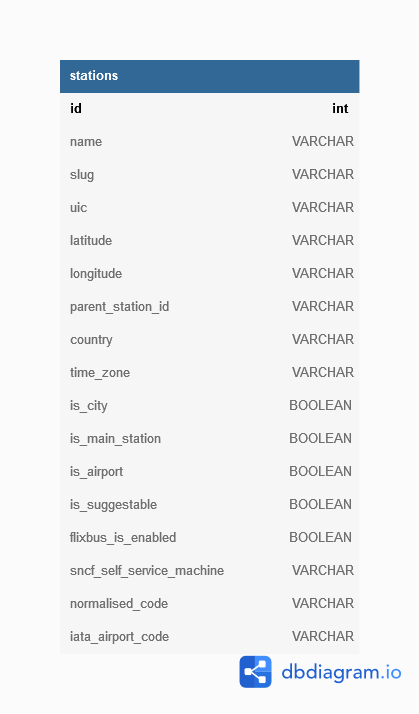
\includegraphics[width=0.35\linewidth]{ERdatabase}
		\caption{Diagramma DB}
		\label{ERdb}
	\end{figure}
	\newpage
	\section{Descrizione degli algoritmi}
	Una volta avviato il programma, all'utente viene richiesto di selezionare i campi di input dagli appositi menù a tendina presenti sull'interfaccia utente. È bene notare, che ogni selezione è strettamente necessaria per elaborazione da parte del programma.\\\\Una volta cliccato il pulsante \verb*|Plan| \verb*|your| \verb*|trip|, verranno avviati tutti gli algoritmi per la definizione dell'itinerario di viaggio.\\\\Inizialmente, nella classe \verb*|FXMLController| vengono effettuate delle verifiche atte a determinare che l'utente abbia selezionato tutti i campi necessari per le operazioni, e se tale controllo non viene superato, nella casella di testo appare un messaggio contenente dei suggerimenti per poter usufruire delle funzionalità (es. Select origin city to continue.). Se tutti i controlli sono superati, seguendo il pattern Model View Controller (MVC), si delega alla classe \verb*|Model| la parte riguardante la logica applicativa. Tale classe richiamerà, quando necessario, la classe \verb*|InterrailDAO| per interrogare il database ed effettuare le operazioni necessarie di estrapolazione dati.\\Dopo aver quindi premuto il pulsante \verb*|Plan| \verb*|your| \verb*|trip|, l'applicazione si collega alla classe \verb*|Model| che crea un grafo nel quale vengono inserite tutte le città contenute nel database: queste città vengono collegate tra di loro con archi solo se la distanza (calcolata tramite la libreria \verb*|LatLngTool| a partire dai dati di longitudine e latitudine) è inferiore al parametro \verb*|TOT| supposto pari a \verb*|1100km|. Tale parametro è modificabile dal programmatore, e tiene conto di alcune considerazioni riguardanti il numero di chilometri verosimilmente percorribili in un giorno di viaggio.\\Successivamente alla creazione del grafo, il programma procede al calcolo tramite algoritmo ricorsivo delle migliori destinazioni a partire dalla città di partenza. In sostanza, l'algoritmo genera a partire dalla città di origine una lista di città prese dalla componente connessa (classe \verb*|ConnectivityInspector|), e da lì viene effettuata la procedura ricorsiva che mira a massimizzare il parametro di riferimento composto dalla somma della statistica relativa al parametro turistico-culturale selezionato dall'utente, prelevato in fase di creazione dell'oggetto \verb*|City| dal database.\\Oltre alla massimizzazione del parametro indicato, l'algoritmo valuta anche la distanza totale percorsa, cercando di minimizzarla il più possibile.\\ Terminata questa fase, la funzione della classe \verb*|Model| che si è occupata di gestire il calcolo delle migliori destinazioni, passa il risultato alla classe \verb*|FXMLController| che fornirà in output all'utente le varie città di destinazione tramite apposita area di testo.
	
	\subsection{Diagramma delle classi principali}
	\begin{figure}[h]
		\centering
		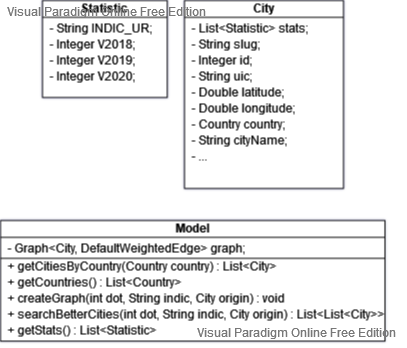
\includegraphics[width=0.7\linewidth]{diagrammaClassiPrincipali}
		\caption{Diagramma delle classi principali}
		\label{diagClassi}
	\end{figure}
	
	\newpage
	\section{Risultati}
	\begin{figure}[h]
		\centering
		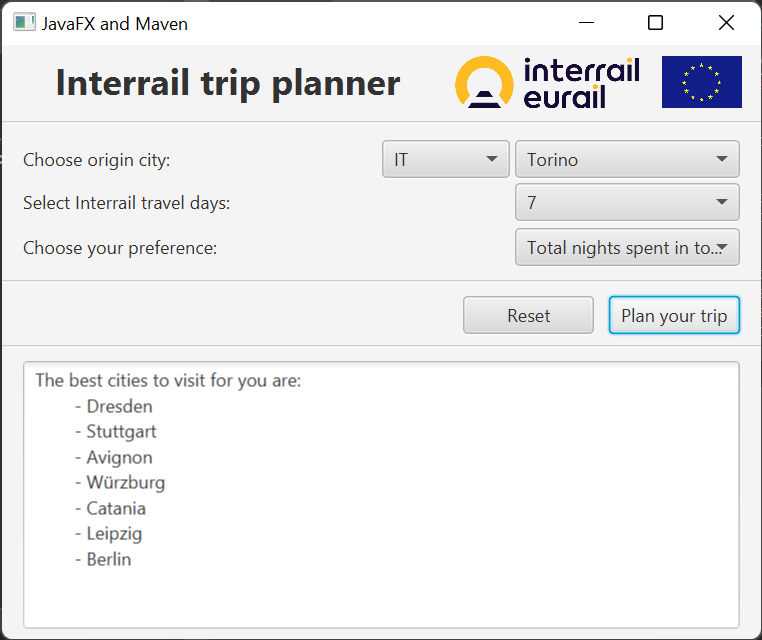
\includegraphics[width=0.5\linewidth]{torino-tur}
		\caption{Torino trip}
		\label{torino-tur}
	\end{figure}
 Nella cattura di figura \ref{torino-tur}, il programma è stato avviato selezionando come città di origine “Torino”, e da lì è stata avviata la ricerca del miglior percorso turistico da effettuare per interessi turistico-culturali orientati al numero di maggiori presenze turistiche.\\\\
	\begin{figure}[h]
		\centering
		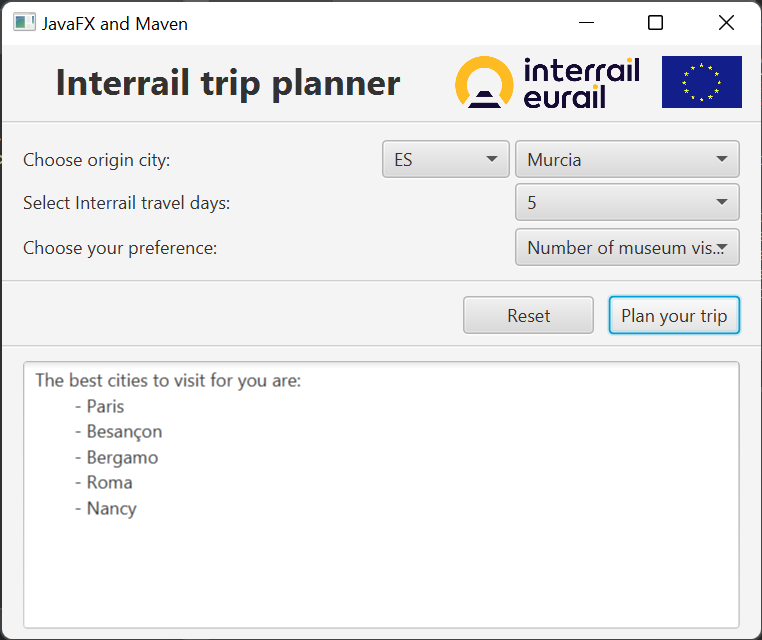
\includegraphics[width=0.5\linewidth]{murcia-mus}
		\caption{Murcia trip}
		\label{murcia-mus}
	\end{figure}
 Nella cattura di figura \ref{murcia-mus}, il programma è stato avviato selezionando come città di origine “Murcia”, e da lì è stata avviata la ricerca del miglior percorso turistico da effettuare per interessi turistico-culturali orientati al numero di maggiori visite presso i musei delle località.\\\\
	\begin{figure}[h]
		\centering
		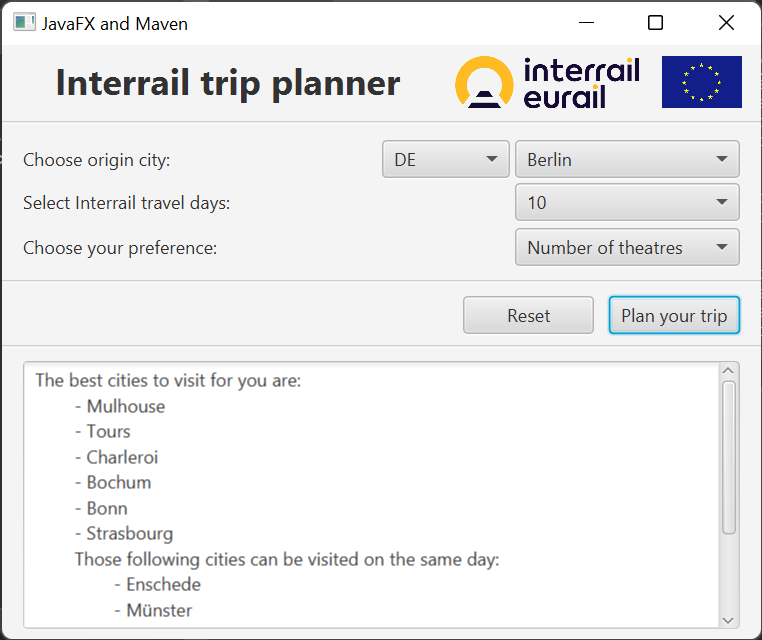
\includegraphics[width=0.5\linewidth]{berlin-the}
		\caption{Berlin trip}
		\label{berlin-the}
	\end{figure}
 Nella cattura di figura \ref{berlin-the}, il programma è stato avviato selezionando come città di origine “Berlino”, e da lì è stata avviata la ricerca del miglior percorso turistico da effettuare per interessi turistico-culturali orientati al numero di opere teatrali.
	
	\subsection{Link al video dimostrativo}
\href{	https://youtu.be/YXR59W2VvJ4 } {Video dimostrativo}
	
	\subsection{Tabella dei risultati ottenuti}
	\begin{tabular}{|c|c|c|c|c|}
		\hline
		Stato & Città & Giorni  & Interesse & Tempo (ms)  \\
		\hline
		IT &Torino  & 7  & Night stays  & 113   \\
		\hline
		DE & Berlin  & 10  & Theatres  & 3523 \\
		\hline
		ES & Murcia  & 5  & Night stays  & 18 \\
		\hline
		FR & Paris  & 5  & Theatres & 15  \\
		\hline
	\end{tabular}

\paragraph{}
Si può notare come al crescere del numero di giorni di viaggio (e quindi del numero di città fornite in output) l'algoritmo fatichi a trovare una soluzione in tempi ristretti. Fino a 7 fornisce soluzione in tempo istantaneo, mentre per valori superiori, l'attesa può anche durare pochi secondi. 
	
	\newpage
	\section{Considerazioni finali}
	\subsection{Punti di forza}
	L'applicazione è molto semplice e permette con estrema rapidità la valutazione di un itinerario turistico basandosi su semplici interessi turistico-culturali.\\L'interfaccia è estremamente intuitiva, e ciò consente anche a utenti poco esperti di poter interfacciarsi con la stessa, senza che vi siano problemi di comprensione circa le funzionalità.\\L'area di testo contenente il contenuto del risultato dell'elaborazione fornisce i risultati in maniera altresì semplice, in modo tale che l'utente possa vedere i nomi delle città immediatamente, senza essere distratto da ulteriori elementi visivi che potrebbero distorcere l'attenzione.\\In caso di input mancante, all'utente viene fornita un'istruzione precisa su come procedere per poter immettere tutte le informazioni necessarie per l'avvio dell'elaborazione.
	\subsection{Limiti} \label{lim}
	I limiti principali dell'applicazione in questione riguardano sicuramente la parte dei dati: essi sono prelevati da due fonti diverse (e già questo di per sé genera problemi di unione dei dati). Inoltre, i dati che concernono il turismo e la cultura nel continente europeo sono poco precisi e vaghi.\\\\L'applicazione presenta anche alcuni limiti della capacità computazionale, che per determinati indicatori e per un numero maggiore o uguale a 10 giorni di viaggio le tempistiche si allungano.
	\subsection{Conclusioni}
	L'applicazione così come si presenta si presta a un utilizzo per ambito non direttamente professionale, per via della sua semplicità e della poca accuratezza dei dati utilizzati.\\L'applicazione si pone come obiettivo la velocizzazione della definizione di itinerari turistici da parte di tour operator e agenzie di viaggio che operino nel settore del turismo e in particolare nella definizione di pacchetti turistici da vendere al dettaglio.\\
	Come risultati, essa fornisce i principali luoghi più affini agli interessi turistici selezionati (considerati i limiti di cui \ref{lim}).\\Un possibile miglioramento può essere apportato alla parte dei dati, poiché i data-set utilizzati non sono stati raccolti in modo completo e uniforme tra i vari Paesi. Inoltre, poiché i dati sul turismo variano quotidianamente, è altresì possibile fornire funzionalità che si occupino di collegamento ai database via rete e del prelievo e analisi dei dati aggiornati. Potendo quindi disporre di strumenti aziendali e dati raccolti da tutto il settore del turismo privato, sicuramente l'applicazione risulterebbe più efficace e completa potendo poi analizzare più fette del mercato turistico.
	
	\newpage
	\section{Licenza d'uso}
	\begin{center}
	 Applicazione Java per il calcolo di un itinerario Interrail © 2022\\ by Filippo Castellarin\\ is licensed under CC BY-NC-SA 4.0 
	\end{center}

\end{document}